\subsection{GTF和GFF文件操作}

\begin{frame}[standout] GTF和GFF文件操作 \end{frame}

\begin{frame}[fragile]{Demo: GFF3 feature}
    % \begin{figure}
    %     \centering
    %     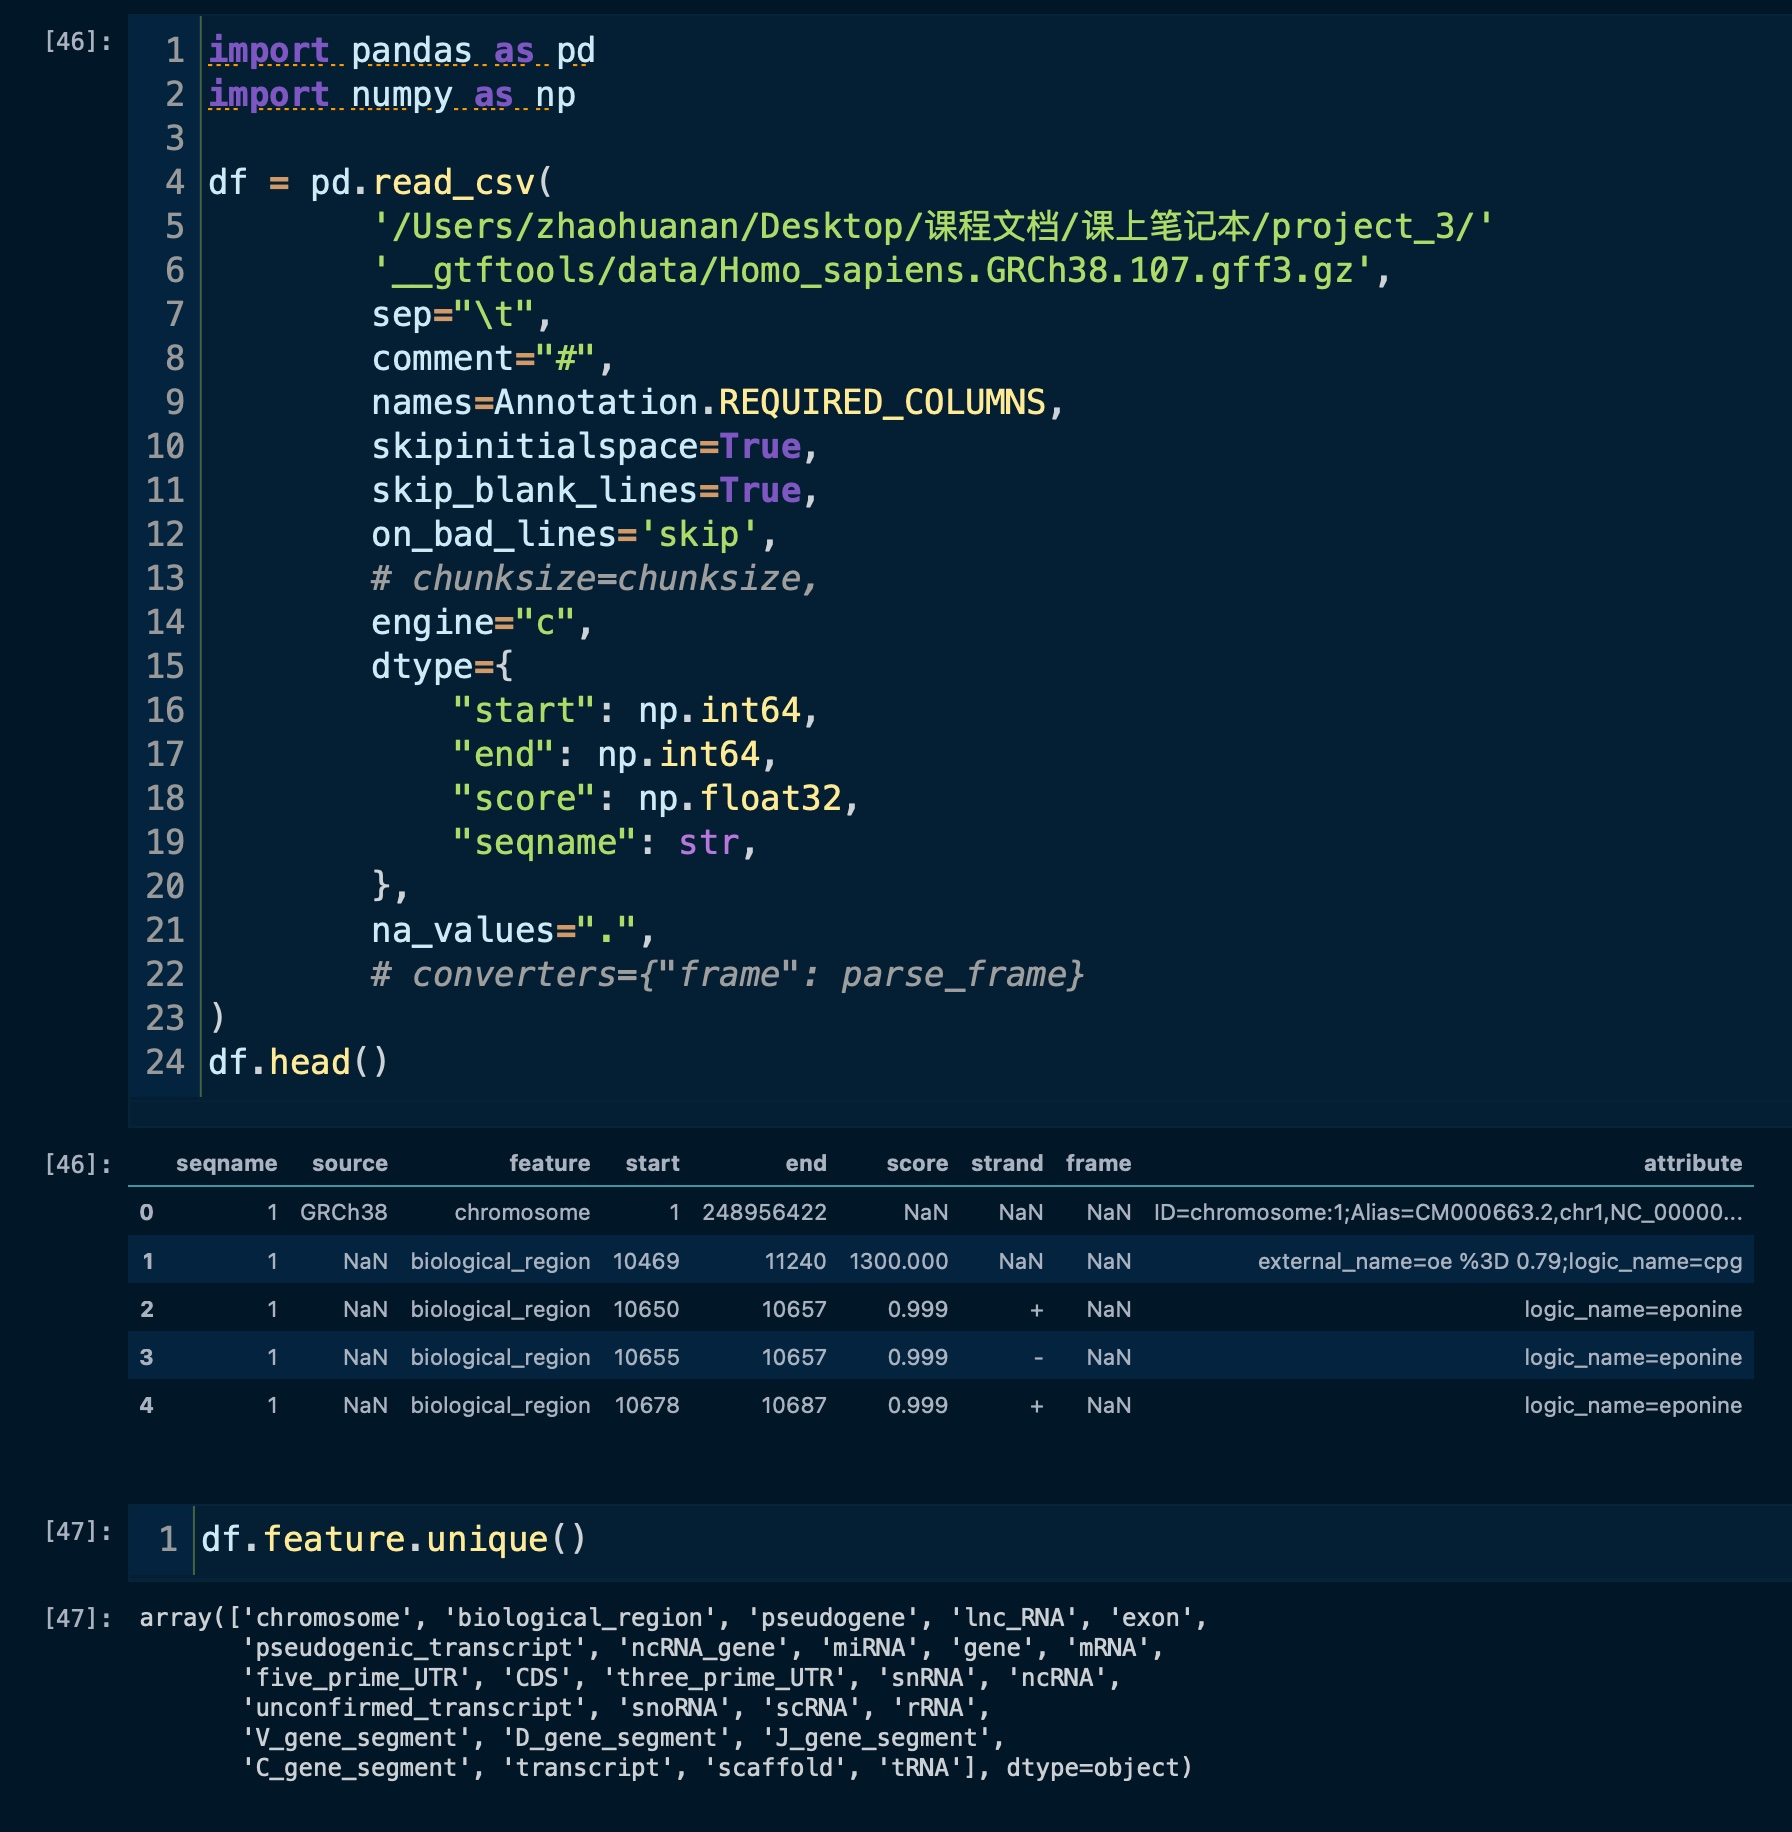
\includegraphics[width=5cm]{Images/gff3_feature.jpg}
    % \end{figure}
    \begin{lstlisting}
import pandas as pd
import numpy as np

df = pd.read_csv(
        'data/Homo_sapiens.GRCh38.107.gff3.gz',
        sep="\t",
        comment="#",
        names=Annotation.REQUIRED_COLUMNS,
        skipinitialspace=True,
        skip_blank_lines=True,
        on_bad_lines='skip',
        # chunksize=chunksize,
        engine="c",
        dtype={
            "start": np.int64,
            "end": np.int64,
            "score": np.float32,
            "seqname": str,
        },
        na_values=".",
)
    \end{lstlisting}
\end{frame}

\begin{frame}[standout] GTF和GFF文件操作 \end{frame}

\begin{frame}[fragile]{Demo: GFF3 feature}
    % \begin{figure}
    %     \centering
    %     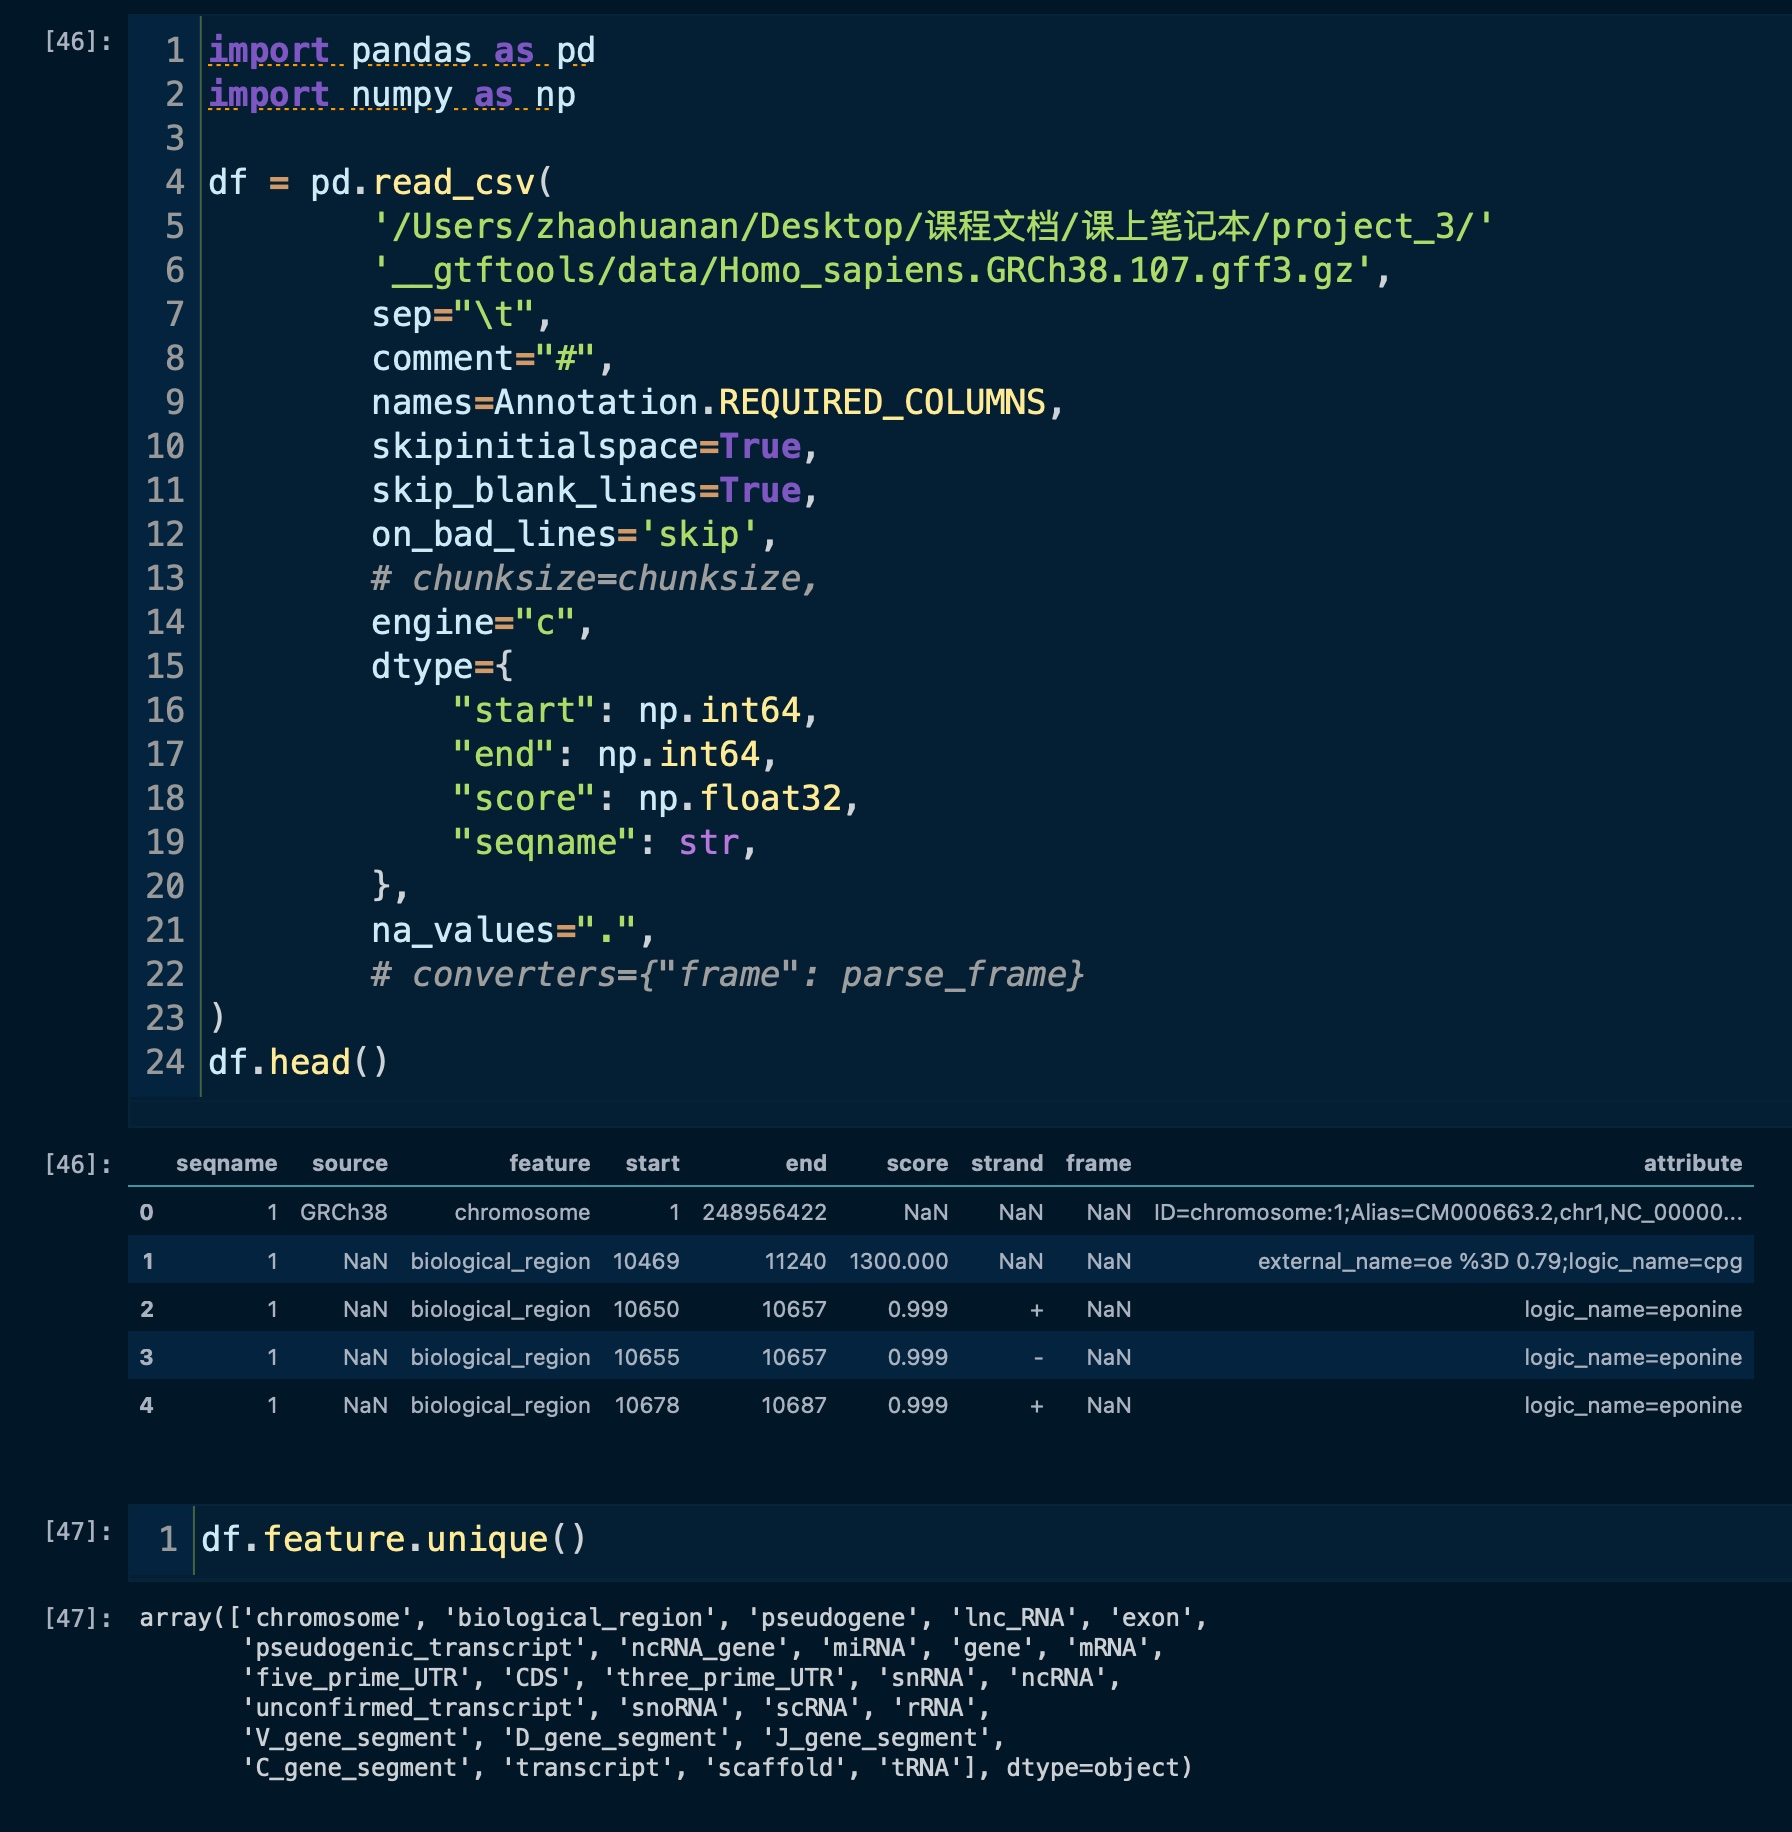
\includegraphics[width=5cm]{Images/gff3_feature.jpg}
    % \end{figure}
    \begin{lstlisting}
df.feature.unique()
array(['chromosome', 'biological_region', 'pseudogene', 'lnc_RNA', 'exon',
       'pseudogenic_transcript', 'ncRNA_gene', 'miRNA', 'gene', 'mRNA',
       'five_prime_UTR', 'CDS', 'three_prime_UTR', 'snRNA', 'ncRNA',
       'unconfirmed_transcript', 'snoRNA', 'scRNA', 'rRNA',
       'V_gene_segment', 'D_gene_segment', 'J_gene_segment',
       'C_gene_segment', 'transcript', 'scaffold', 'tRNA'], dtype=object)

# feature required: 
# - "CDS", 
# - "start_codon"  # 简化,先不考虑,其实是CDS前三个碱基
# - "stop_codon"  # 简化,先不考虑

# optional:
# - "5UTR", 
# - "3UTR",
# - "*RNA"
    \end{lstlisting}
\end{frame}


\begin{frame}[fragile]{练习}
    \begin{lstlisting}
- 仅在必要时才对 self 或 cls 注释(实战课三当中进行讲解)
- cls + @classmethod
- GFF与GTF文件进行转换

- 统计各条染色体的基因密度
- 获得基因的的TSS, TES及启动子坐标 (GFF3)
- 计算全基因组可转录区域长度及所占基因组比例 (GFF3, GTF)
- 计算基因的转录长度、外显子数目及翻译区长度 (GFF3)
    - 计算基因的转录长度
        - 统计平均长度,中位数长度
    - 计算基因的外显子(exon)个数
        - 统计平均个数,中位数个数
        - 统计最多exon的基因, 最少exon的gene
- 程序 CLI 化
    - sys.argv
    - argparse
    \end{lstlisting}
\end{frame}